\documentclass[twoside]{uva-inf-bachelor-thesis}
\usepackage[english]{babel}

% Filling your thesis with only lorem ipsum is not advised.
\usepackage{lipsum}

\usepackage{amsthm}

\theoremstyle{definition}
\newtheorem{definition}{Definition}[section]


% \usepackage{cite}
\usepackage[style=authoryear-comp]{biblatex}
\addbibresource{Project/Thesis/LaTeX/main.bib}

% Title Page
\title{Development of an interactive experiment on the effect of sequential information on the formation of generic beliefs}
\author{Bodi Boelé}
\supervisors{Dr. Patricia Mirabile}
\signedby{-}

\begin{document}
\maketitle

\begin{abstract}
Building on earlier (ongoing) investigations on generics and alternatives, this paper will discuss the online implementation of a (dedicated) tool to host an interactive experiment and then use this tool to execute a pilot experiment.

Generic statements are statements such as `ducks lay eggs', `tigers are striped', `lions have manes' and `ticks spread Lyme disease'. They express generalizations about the members of a kind. The statements mentioned lack any form of quantification and are therefore `bare'. 
\end{abstract}

\tableofcontents

\chapter{Introduction}
\section{Generic statements}
Generic statements are sentences which we use to attribute features, patterns, sentiments and other beliefs to a group.
`Ducks lay eggs', `tigers are striped', `lions have manes' and `ticks spread Lyme disease' are examples of generic statements. Generics statements express generalizations about the members of a kind. The given examples lack any form of quantification and are therefore `bare'. Other than bare, there are also other types of generic statements, such as a quantified statement, `all ducks lay eggs' and `all tigers are striped'. This research will however focus on `Bare generics'.

`Bare' generic statements express useful generalizations, but an unambiguous conclusion on when people think these statements are true can not be formed. There is no unique critical point of statistical prevalence of the feature in the kind where people in general tend to designate a statement as true. For example when people have to judge the statement `lions have manes', the predominant judgement will be that the statement is true, although less than 50\% of lions (only the older male lions) have manes. When asked about the statement `ticks spread Lyme disease' the predominant conclusion as well would be true, even though the statement is only true for 2.7\% \parencite{rivm_2019} of tick bites that actually transfer the disease whereas 20\% of ticks carry the disease. These rather large differences in truth-conditions as investigated by \cite{leslie2011all} can be partly devoted to the generic overgeneralization effect.

\section{Statistical and Emperical research}
There are two main types of research on generics, empirical and statistical research. Empirical research is based on the scientific method of inquiry and observation through experiments. This means personal beliefs and biases need to be kept out of the equation from actual experiments. You should draw conclusions based on empirical data and not what your gut feeling says. Empirical research focuses on preferences.

Statistical research involves defining phenomena in terms of numbers, development and application of theory and methods, statistical analysis and the analysis of research data. The focus is on formal rules and proving the correctness of a rule.

In generics these approaches are closely related and intertwined with each other. The ideal case is that the statistical research can be acknowledged using empirical data. 

The statistical approach is criticised by many because of the idea that any formal rule should be based on probabilistic considerations, which makes it impossible to take into account the mismatch between thoughts of people and the probability given.

\section{Goal}
The goal of this research project is to implement an interactive experiment which enables investigation of the effect of sequential information on the semantics of generic statements. The focus of this experiment will be on the importance of the learning process on the formation of beliefs regarding generic statements. This project seeks to implement an online tool which will first be tested using a pilot experiment. As a follow up the tool will used in an ongoing research project by \cite{RooijSchulzGenAlt} on `Generics and Alternatives`. In their research \cite{RooijSchulzGenAlt} use a statistical approach to the meaning of generic sentences. Their paper discusses 3 studies that tested their proposal. They presented participants, who were recruited through Prolific, with a visual stimuli and asked to judge the assertability of a generic sentence describing the stimuli.  In their conclusion they mention two shortcomings of their research that should be the focus of future work. The shortcomings mentioned are that the experiment did not take into the learning phase of the participant and the second is that the experiment did not account for what the participant considered a relevant alternative. The first shortcoming is where this thesis ties in with the investigation. This to be able to add ground to build a solid basis from where further theoretical work can be directed.

\chapter{Theoretical background}
The main approach to statistical analysis of generic sentences is the use of the majority rule. Assuming a sentence `tigers are striped' (form: `Gs are f') the majority rule for a generic sentence is defined as:
\theoremstyle{definition}
\begin{definition}
A generic sentence of the form `Gs are f' is true i.f.f. $P(f|G) > \frac{1}{2}$
\end{definition}
The majority rule has various shortcomings, such as the `ticks' example mentioned in the introduction. With 2.7\% this statement should come back as false, by definition of the majority rule, but somehow participants chose otherwise. In their paper \cite{RooijSchulzGenAlt} suggest that the reason people were not finding acceptance because they were only looking at majority rules and discuss that by taking into account various notions of alternatives, many shortcomings of the majority rule can be overcome, by compensating for different factors.

\cite{van2020generics} based their analysis of generic statements on the majority rule, the intuition that other authors had formed over the years and claimed to be natural. In their paper they suggest that people tend to accept and interpret generics based on a distorted picture of it provided by the media instead of on actual frequencies.


\subsection{Overgeneralization effect}
Experimental psychology has highlighted a number of biases and preferences such as the generic overgeneralization effect, the bias for people to accept a generic statement based on rare events and the biased position of people where they are more negatively biased towards non-human categories. For example people tend to classify `Men attack people' as false and `Sharks attack people' as true, even though the chance of men attacking people is vastly higher than the chance of sharks attacking people. 

A bare generic statement, `ducks lay eggs' appears to be true, even though it is physically impossible for male ducks.
The universally quantified version of this generic statement should be rejected by it's incorrectness; `All ducks lay eggs' can not be true since many ducks do not lay eggs. \cite{leslie2011all} set out different experiments focusing on the semantics of this phenomena. In one of their experiments they found that, despite knowing the relevant information, the universal statements would often be judged true. In another experiment they offered the participant a correct alternative statement to the bare generic statement and even then the participants would hold on to the `overgeneralized' statement. Their research shows that people tend to falsely accept (over)generalized statements when offered a more descriptive alternative, as described in the previous section. 

Experiments done by \cite{tasimi2017differences} indicate that people are negatively biased towards generics involving non-human entities. In different experiments participants were assigned a domain, either people or tools/things. The overarching research project of this thesis is about formation of generic beliefs and therefor it is important to acknowledge the possibility of such a bias during the investigation.

\subsection{Impact on generic beliefs}
Experimental evidence that whether a generic statement is true does not depend on underlying statistics dates back to as early as 1966 by \cite{gilson1965subjective}. According to \cite{cimpian2010generic} `generic statements require little evidence for acceptance' such as the previously mentioned tick example and other striking generics like `Rottweilers maul children' and `Lions eat people' who appear as true, even though these statements are only true for exceptional cases. According to their research generic statements are often judged as true based on little evidence, but these implications go far beyond what is needed to accept them. Using the `ticks spread Lyme disease' example, people tend to believe that all ticks spread Lyme disease and therefor people tend to be more afraid of ticks than you would expect from a statistical point of view. Another example is the fear of Rottweilers or the assumption that flying as a means of transport is unsafe. The influence of information and how this is interpreted, and how magnifying rare events paints an incomplete picture on which people base their judgement, as suggested by \cite{van2020generics}. This underlines the importance of the parent research on how people form generic beliefs and what the effect of sequential information is on their judgement. 

\section{Hypothesis}

\chapter{Methods}
\section{Experimental Setup}
This experiment builds on the basis created by \cite{RooijSchulzGenAlt}. In their experiment they show the contestant a grid consisting of 2 differently coloured bugs, as shown in \ref{fig:beetle_example}. The contestant is able to rate the generic statement using a continuous scale.
\begin{figure}[h]
    \centering
    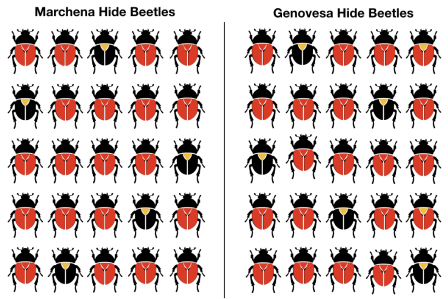
\includegraphics[width=0.7\textwidth]{Project/Thesis/LaTeX/images/beetles_example.png}
    \caption{Sample of experiments done by \cite{RooijSchulzGenAlt} as seen by the contestant}
    \label{fig:beetle_example}
\end{figure}
To be able to investigate the influence of sequential data on the semantics, we used a set-up similar to that of the previous experiment as shown in \ref{fig:beetle_example}. The interactive implementation has a similar appearance, except that the field will be initialised as a board consisting of tiles, somewhat resembling a game of memory. The user must interact with the interface and sequentially turn around all tiles on the user's side of the board, one by one, before being able to rate the presented statement. An example of this board is given in \ref{fig:beetle_example_mem}. 
\begin{figure}[h]
    \centering
    % \includegraphics[width=0.7\textwidth]{TODO}
    \caption{Sample of the experiments set-up}
    \label{fig:beetle_example_mem}
\end{figure}
The experiment allows the contestant to have a sequential learning process.

\section{Implementation}

\section{Data collection plan}
Data for this thesis will be collected in a pilot experiment using the interactive web questionnaire created for this purpose. Participants for this pilot experiment will be recruited using social media connections, to also be able to receive feedback on the questionnaire itself.

The extended experiment will recruit participants via Prolific.ac, an online platform aimed
at connecting researchers and participants willing to fill in surveys and questionnaires in exchange for compensation for their time \cite{PALAN201822}.



\chapter{Results}
\section{Gathering data}
\subsection{Experimental set-up}


\chapter{Discussion}
\section{Ethical aspects}

\chapter{Conclusions}

\printbibliography
\addcontentsline{toc}{chapter}{Bibliography}

\end{document}
